\documentclass[../Languages.tex]{subfiles}

\begin{document}
\usec{Scala}\label{sec:scala}

\cd{Scala} is a general-purpose programming language providing support for
functional programming and a strong static type stream. Designed to be concise,
many of \cd{Scala}'s design decisions aimed to address criticisms of \cd{Java}.

\cd{Scala} source code is intended to be compiled to \cd{Java} bytecode, so
that the resulting executable code runs on a \cd{Java} virtual machine.
\cd{Scala} provides languages interoperability with \cd{Java}, so that
libraries written in both languages may be referenced directly in \cd{Scala} or
\cd{Java} code. Like \cd{Java}, \cd{Scala} is object-oriented, and use a
curly-brace syntax reminiscent of the \cd{C} programming languages like
\cd{Scheme}, \cd{Standard ML} and \cd{Haskell}, including currying, type
interface, immutability, lazy evaluation, and pattern matching. It also has an
advance type system supporting algebraic data types, covariance and
contravariance, higher-order types (but not higher-rank types), and anonymous
types. Other features of \cd{Scala} not present in \cd{Java} include operator
overloading, optional parameters, named parameters, and raw strings.
Conversely, a features of \cd{Java} not \cd{Scala} is checked exceptions, which
have proved controversial.

The name \cd{Scala} is a portmanteau of \textit{scalable} and
\textit{language}, signifying that it is designed to grow with the demands of
its users. 

\subsection{Influence}\label{sub:influence}

\begin{Figure}
  \centering
  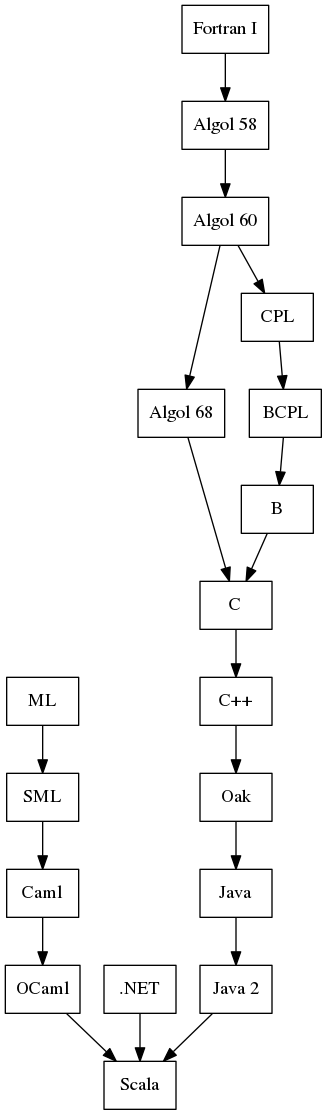
\includegraphics[height=0.5\textheight]{scala}
  \captionof{figure}{Inheritance diagram for \cd{Scala}.}
\end{Figure}

\newpage
\end{document}
